        %%******************************************%%
        %%                                          %%
        %%        Modello di tesi di laurea         %%
        %%            di Andrea Giraldin            %%
        %%                                          %%
        %%             2 novembre 2012              %%
        %%                                          %%
        %%******************************************%%

\begin{document}
    \frontmatter
    \begin{titlepage}
    \begin{center}
        \begin{LARGE}
            \textbf{\myUni}\\
        \end{LARGE}

        \vspace{10pt}

        \begin{Large}
            \textsc{\myDepartment}\\
        \end{Large}

        \vspace{10pt}

        \begin{large}
            \textsc{\myFaculty}\\
        \end{large}

        \vspace{30pt}
        \begin{figure}[htbp]
            \centering
            
\includegraphics[height=6cm]{images/unipd-logo.png}
        \end{figure}
        \vspace{30pt}

        \begin{LARGE}
            \textbf{\myTitle}\\
        \end{LARGE}

        \vspace{10pt}

        \begin{large}
            \textsl{\myDegree}\\
        \end{large}

        \vspace{40pt}

        \begin{large}
            \begin{flushleft}
                \textit{Relatore}\\
                \vspace{5pt}
                \profTitle\ \myProf
            \end{flushleft}

            \vspace{-52pt}

            \begin{flushright}
                \textit{Laureando}\\
                \vspace{5pt}
                \myName \\
                \vspace{5pt}
                \textit{Matricola} \myID
            \end{flushright}
        \end{large}

        \vspace{40pt}

        \line(1, 0){338} \\
        \begin{normalsize}
            \textsc{Anno Accademico \myAA}
        \end{normalsize}
    \end{center}
\end{titlepage}

    \clearpage
\phantomsection
\thispagestyle{empty}

\hfill
\vfill

\noindent\myName: \textit{\myTitle,}
\myDegree,
\textcopyright\ \myTime.

    %\cleardoublepage
\phantomsection
\thispagestyle{empty}
\pdfbookmark{Dedica}{Dedica}

\vspace*{3cm}

\begin{center}
    \textit{Lorem ipsum dolor sit amet} \\ \medskip
    --- Lorem ipsum
\end{center}

\medskip

    \cleardoublepage
\phantomsection
\pdfbookmark{Sommario}{Sommario}
\begingroup
\let\clearpage\relax
\let\cleardoublepage\relax
\let\cleardoublepage\relax

\chapter*{Sommario}

Il presente documento descrive il lavoro svolto durante lo \textit{stage} curriculare svolto presso VISIONEIMPRESA s.r.l. Società Benefit di Pernumia (PD).\\
L'obiettivo principale dello \textit{stage} era l'aggiornamento dell'applicazione \textit{mobile} moviEXPENSE, precedentemente sviluppata da VISIONEIMPRESA per facilitare e velocizzare la registrazione delle note spese, in modo da ridurre la quantità di documenti cartacei prodotti e i tempi di attesa per la ricezione dei dati da parte del personale amministrativo dell'azienda utilizzatrice.\\
L'aggiornamento riguardava in particolare la sicurezza dell'applicazione, in quando le stringhe di connessione ai database venivano trasmesse in chiaro, la correzione di \textit{bug}, l'implementazione di nuove funzionalità e il miglioramento di quelle già presenti, e, infine, il \textit{restyling} dell'interfaccia grafica.

\endgroup

\vfill

    %\cleardoublepage
\phantomsection
\pdfbookmark{Ringraziamenti}{ringraziamenti}

\bigskip

\begingroup
\let\clearpage\relax
\let\cleardoublepage\relax
\let\cleardoublepage\relax

\chapter*{Ringraziamenti}

Ringrazio innanzitutto il professor Francesco Ranzato, relatore della tesi, per la disponibilità e la rapidità nella comunicazione.\\

\noindent Desidero ringraziare Francesco Turra e tutta VISIONEIMPRESA per avermi dato l'opportunità di svolgere lo \textit{stage} in tempi rapidi e compatibili con la presente sessione di laurea.\\

\noindent Ringrazio anche la mia famiglia e in particolare i miei genitori per il supporto, anche economico, datomi durante questi tre anni.\\

\noindent Un ringraziamento va anche ai compagni di corso che ho conosciuto, in particolare al gruppo \textit{Error\_418}, ottimi compagni di lavoro durante il progetto di ingegneria del \textit{software}.\\

\noindent Ringrazio ovviamente i miei amici Marta e Gianmarco, che mi hanno sempre supportato, spingendomi ad andare sempre avanti in qualsiasi situazione, soprattutto grazie ai \textit{sushi} post sessione.\\

\noindent Infine vorrei ringraziare anche tutti gli amici trovati e ritrovati in questi tre anni, che hanno contribuito ad alleggerire il percorso che si sta ora concludendo.\\

\bigskip

\noindent\textit{\myLocation, \myTime}
\hfill \myName

\endgroup

    \cleardoublepage
\pdfbookmark{\contentsname}{tableofcontents}
\setcounter{tocdepth}{2}
\tableofcontents
%\markboth{\contentsname}{\contentsname}
\clearpage

\begingroup
    \let\clearpage\relax
    \let\cleardoublepage\relax
    \let\cleardoublepage\relax

    % Figures list
    \phantomsection
    \pdfbookmark{\listfigurename}{lof}
    \listoffigures

    \vspace*{8ex}

    % Tables list
    \phantomsection
    \pdfbookmark{\listtablename}{lot}
    \listoftables

    \vspace*{8ex}
\endgroup
\cleardoublepage

    \cleardoublepage

    \mainmatter
    \chapter{Introduzione}
\label{cap:introduzione}

\section{Convenzioni tipografiche}

Durante la stesura del documento sono state adottate le seguenti convenzioni tipografiche:
\begin{enumerate}
    \item i termini tecnici, non di uso comune, ambigui, oltre che gli acronimi e le abbreviazioni, sono stati definiti nel glossario situato al termine del presente documento;
    \item la prima occorrenza di ogni termine presente nel glossario viene identificata nel seguente modo: \emph{termine di glossario}\glsfirstoccur;
    \item i termini in lingua inglese sono riportati in \textit{corsivo}.
\end{enumerate}

\section{L'azienda}

\begin{figure}[!h]
    \centering 
    
\includegraphics[width=0.6\columnwidth]{images/logo-visioneimpresa.png} 
    \caption{Logo di VISIONEIMPRESA s.r.l. Società Benefit}
\end{figure}
\noindent VISIONEIMPRESA s.r.l. è una \textit{software house} nata negli anni Ottanta a Pernumia, in provincia di Padova. Dal 2016 fa parte di Office Group, un gruppo nato dall'unione di Office Information Technologies di Montegrotto Terme con altre aziende di Veneto e Lombardia.\\
L'obiettivo di VISIONEIMPRESA è lo sviluppo e la vendita di software gestionali per agevolare il lavoro delle piccole e medie aziende e contribuire alla loro digitalizzazione. I software sviluppati si dividono principalmente in due gruppi:
\begin{itemize}
    \item \textbf{software Vision}: il software principale è VisionEnterprise, ideato per migliorare la gestione dell'organizzazione aziendale nel suo complesso. In questo gruppo di software rientrano le soluzioni verticali, gestionali per specifiche tipologie di aziende, ad esempio VisionENERGY per il commercio di prodotti petroliferi o VisionFRESH per l'ingrosso di prodotti ortofrutticoli;
    \item \textbf{software movi}: applicazioni mobile specializzate in determinate azioni, ad esempio l'analisi dati (moviCHECK), l'invio di ordini (moviORDER) o l'invio di ticket per l'assistenza post-vendita (moviTICKET).
\end{itemize}
\noindent Nel 2023 VISIONEIMPRESA s.r.l. è diventata anche \gls{Società Benefit}\glsfirstoccur, impegnandosi così a perseguire obiettivi tra i quali rientrano il mantenimento di un buon equilibrio tra vita personale e lavoro dei dipendenti e la collaborazione con istituti di formazione del territorio (scuole superiori e università).

\section{Struttura del documento}

% TODO rivedere

\begin{description} 
    \item[{\hyperref[cap:descrizione-stage]{Il secondo capitolo}}] descrive il progetto di stage e lo scopo dell'applicazione.
    
    \item[{\hyperref[cap:tecnologie-strumenti]{Il terzo capitolo}}] presenta gli strumenti e le tecnologie utilizzate durante lo stage.
    
    \item[{\hyperref[cap:design]{Il quarto capitolo}}] descrive l'architettura e dell'applicazione.
    
    \item[{\hyperref[cap:codifica]{Il quinto capitolo}}] espone le principali modifiche effettuate e novità apportate, concludendo con una breve descrizione delle attività di verifica e validazione.
    
    \item[{\hyperref[cap:conclusioni]{Il sesto capitolo}}] espone le conclusioni tratte dall'esperienza di stage.
\end{description}

    \chapter{Descrizione dello stage}
\label{cap:descrizione-stage}

\intro{Breve introduzione al capitolo}\\

\section{Introduzione al progetto}

\section{Analisi preventiva dei rischi}

Durante la fase di analisi iniziale sono stati individuati alcuni possibili rischi a cui si potrà andare incontro.
Si è quindi proceduto a elaborare delle possibili soluzioni per far fronte a tali rischi.\\

\begin{risk}{Performance del simulatore hardware}
    \riskdescription{le performance del simulatore hardware e la comunicazione con questo potrebbero risultare lenti o non abbastanza buoni da causare il fallimento dei test}
    \risksolution{coinvolgimento del responsabile a capo del progetto relativo il simulatore hardware}
    \label{risk:hardware-simulator} 
\end{risk}

\section{Requisiti e obiettivi}


\section{Pianificazione}

    \chapter{Strumenti e tecnologie}
\label{cap:strumenti-tecnologie}

\intro{Brevissima introduzione al capitolo}\\

\section{Strumenti}


\section{Strumenti}

    \chapter{Analisi dei requisiti}
\label{cap:analisi-requisiti}

\intro{Breve introduzione al capitolo}\\

\section{Casi d'uso}

Per lo studio dei casi di utilizzo del prodotto sono stati creati dei diagrammi.
I diagrammi dei casi d'uso (in inglese \emph{Use Case Diagram}) sono diagrammi di tipo \gls{uml} dedicati alla descrizione delle funzioni o servizi offerti da un sistema, così come sono percepiti e utilizzati dagli attori che interagiscono col sistema stesso.
Essendo il progetto finalizzato alla creazione di un tool per l'automazione di un processo, le interazioni da parte dell'utilizzatore devono essere ovviamente ridotte allo stretto necessario. Per questo motivo i diagrammi d'uso risultano semplici e in numero ridotto.

\begin{figure}[!h] 
    \centering 
    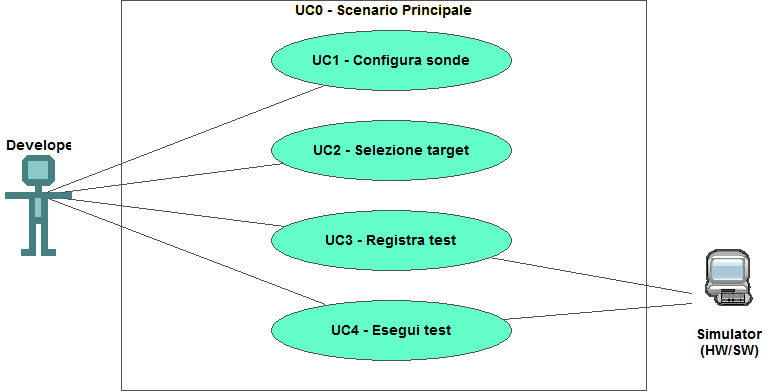
\includegraphics[width=0.9\columnwidth]{images/usecase/scenario-principale} 
    \caption{Use Case - UC0: Scenario principale}
\end{figure}

\begin{usecase}{0}{Scenario principale}
\usecaseactors{Sviluppatore applicativi}
\usecasepre{Lo sviluppatore è entrato nel plug-in di simulazione all'interno dell'IDE}
\usecasedesc{La finestra di simulazione mette a disposizione i comandi per configurare, registrare o eseguire un test}
\usecasepost{Il sistema è pronto per permettere una nuova interazione}
\label{uc:scenario-principale}
\end{usecase}

\section{Tracciamento dei requisiti}

Da un'attenta analisi dei requisiti e degli use case effettuata sul progetto è stata stilata la tabella che traccia i requisiti in rapporto agli use case.\\
Sono stati individuati diversi tipi di requisiti e si è quindi fatto utilizzo di un codice identificativo per distinguerli.\\
Il codice dei requisiti è così strutturato R(F/Q/V)(N/D/O) dove:
\begin{enumerate}
	\item[R =] requisito
    \item[F =] funzionale
    \item[Q =] qualitativo
    \item[V =] di vincolo
    \item[N =] obbligatorio (necessario)
    \item[D =] desiderabile
    \item[Z =] opzionale
\end{enumerate}
Nelle tabelle \ref{tab:requisiti-funzionali}, \ref{tab:requisiti-qualitativi} e \ref{tab:requisiti-vincolo} sono riassunti i requisiti e il loro tracciamento con gli use case delineati in fase di analisi.

\newpage

\begin{table}%
\caption{Tabella del tracciamento dei requisti funzionali}
\label{tab:requisiti-funzionali}
\begin{tabularx}{\textwidth}{lXl}
\hline\hline
\textbf{Requisito} & \textbf{Descrizione} & \textbf{Use Case}\\
\hline
RFN-1     & L'interfaccia permette di configurare il tipo di sonde del test & UC1 \\
\hline
\end{tabularx}
\end{table}%

\begin{table}%
\caption{Tabella del tracciamento dei requisiti qualitativi}
\label{tab:requisiti-qualitativi}
\begin{tabularx}{\textwidth}{lXl}
\hline\hline
\textbf{Requisito} & \textbf{Descrizione} & \textbf{Use Case}\\
\hline
RQD-1    & Le prestazioni del simulatore hardware deve garantire la giusta esecuzione dei test e non la generazione di falsi negativi & - \\
\hline
\end{tabularx}
\end{table}%

\begin{table}%
\caption{Tabella del tracciamento dei requisiti di vincolo}
\label{tab:requisiti-vincolo}
\begin{tabularx}{\textwidth}{lXl}
\hline\hline
\textbf{Requisito} & \textbf{Descrizione} & \textbf{Use Case}\\
\hline
RVO-1    & La libreria per l'esecuzione dei test automatici deve essere riutilizzabile & - \\
\hline
\end{tabularx}
\end{table}%

    \chapter{Progettazione e codifica}
\label{cap:progettazione-codifica}

\intro{Breve introduzione al capitolo}\\

\section{Tecnologie e strumenti}
\label{sec:tecnologie-strumenti}

Di seguito viene data una panoramica delle tecnologie e strumenti utilizzati.

\subsection*{Tecnologia 1}
Descrizione Tecnologia 1.

\subsection*{Tecnologia 2}
Descrizione Tecnologia 2

\section{Ciclo di vita del software}
\label{sec:ciclo-vita-software}

\section{Progettazione}
\label{sec:progettazione}

\subsubsection{Namespace 1} %**************************
Descrizione namespace 1.

\begin{namespacedesc}
    \classdesc{Classe 1}{Descrizione classe 1}
    \classdesc{Classe 2}{Descrizione classe 2}
\end{namespacedesc}


\section{Design Pattern utilizzati}

\section{Codifica}

    \chapter{Verifica e validazione}
\label{cap:verifica-validazione}

    \chapter{Conclusioni}
\label{cap:conclusioni}

\intro{In questo capitolo vengono presentate le conclusioni tratte da questa esperienza di \textit{stage}. La prima parte del capitolo si concentra sull'organizzazione e gli obiettivi del progetto, mentre la seconda parte è incentrata sulle riflessioni svolte a termine dell'esperienza.}

\section{Consuntivo orario}

\renewcommand{\arraystretch}{1.3}
\begin{table}[H]
    \centering
        \begin{tabular}{| c | c | c | c |} 
        \hline
        \textbf{Settimana} & \textbf{Attività} & \textbf{Ore} & \textbf{Variazione}\\
        \hline
        1 & Studio & 50 & +10 \\ 
        \hline
        2 & Autenticazione & 40 & - \\
        \hline
        3-4-5 & \emph{Bug fixing} e novità & 120 & - \\
        \hline
        6 & Interfacce & 40 & - \\
        \hline
        7-8 & Test e documentazione & 50 & -10\\
        \hline
        \multicolumn{4}{c}{\rule{0pt}{1em}} \\
        \hline
        \multicolumn{2}{|c|}{\textbf{Totale}} & 300 & $\pm$0\\
        \hline
        \end{tabular}
        \caption{Consuntivo del lavoro per settimane e ore}
\end{table}
\renewcommand{\arraystretch}{1}

\noindent Come si può notare dalla tabella, ci sono state delle piccole variazioni nel numero di ore di alcune attività, ma queste non sono andate ad influenzare il monte ore finale.\\
Per quanto riguarda, invece, la distribuzione di tali attività nelle settimane, "\emph{bug fixing}" e "novità" sono state inserite nella stessa riga, occupando le settimane dalla 3 alla 5. Questo perché le due attività sono state svolte insieme, e non in modo sequenziale, in quanto l'implementazione delle richieste sull'applicazione ha seguito l'ordine presente nel documento in cui tali richieste erano esposte, nel quale non era presente una divisione netta tra le richieste di \emph{bug fixing} e di introduzione di novità.\\
La prima settimana di lavoro è durata più di quanto pianificato perché la configurazione dell'applicazione per la sua esecuzione in locale ha richiesto più tempo del previsto.

\section{Obiettivi raggiunti}

Al termine dello \textit{stage} ho raggiunto tutti gli obiettivi obbligatori esposti nella \sezref{cap:obiettivi} e quasi tutti i desiderabili. Le uniche due attività non svolte sono state la creazione del manuale utente dell'applicazione e la rivisitazione dell'interfaccia grafica per uso su \emph{tablet}, a causa di mancanza di tempo, ma dato che avevano entrambe una bassa priorità, il livello di soddisfazione da parte dell'azienda è stato comunque alto.\\
Di seguito è riportata una tabella con le percentuali di raggiungimento degli obiettivi.

\renewcommand{\arraystretch}{1.3}
\begin{table}[H]
    \centering
        \begin{tabular}{| c | c |} 
        \hline
        \textbf{Categoria obiettivi} & \textbf{Percentuale di raggiungimento}\\
        \hline
        Obbligatori & 100\% \\
        \hline
        Desiderabili & 75\% \\
        \hline
        Opzionali & 0\% \\
        \hline
        \multicolumn{2}{c}{\rule{0pt}{1em}} \\
        \hline
        \textbf{Totale} & 83,33\%\tablefootnote{Ho utilizzato il numero di obiettivi di ogni categoria come "peso" per il calcolo della percentuale totale.$$P_{tot}=\frac{n_1P_1+n_2P_2+n_3P_3}{n_1+n_2+n_3}=\frac{7\cdot100+4\cdot75+1\cdot0}{7+4+1}=83,33$$} \\
        \hline
        \end{tabular}
        \caption{Percentuali di raggiungimento obiettivi per categorie}
\end{table}
\renewcommand{\arraystretch}{1}


\section{Conoscenze acquisite}

Grazie a questo \textit{stage} ho potuto affacciarmi al mondo della programmazione \textit{mobile}, argomento che non avevo trattato né all'università e nemmeno individualmente, poiché non mi attirava in modo particolare. In questo contesto ho migliorato le mie capacità di autoapprendimento legate sia allo studio di nuovi strumenti e tecnologie che all'utilizzo e lo studio di software realizzato da altri, comprendendone l'architettura, l'organizzazione delle cartelle e lo stile di codifica.\\
Benché il \textit{framework} utilizzato per il \textit{frontend} (Xamarin) non sia più supportato, ho comunque ritenuto utile il suo studio, in quanto è in ogni caso la base di partenza per il \textit{framework} che l'ha sostituito, ovvero .NET MAUI, e perciò se in futuro mi verrà chiesto di sviluppare applicazioni utilizzando questo nuovo \textit{framework}, avrò già una conoscenza di base che mi permetterà di apprenderlo più facilmente.


\section{Valutazione personale}

Nel complesso ho ritenuto lo \textit{stage} un'esperienza molto utile, in quanto mi ha permesso innanzitutto di interfacciarmi con il mondo del lavoro, in particolare con la "vita d'ufficio", esperienza che non avevo mai svolto. Ritengo quindi importante anche lo svolgimento di un'esperienza di questo tipo in presenza piuttosto che da remoto, specialmente se è la prima esperienza lavorativa che si affronta, in quanto la comunicazione con i colleghi risulta più rapida ed efficiente rispetto ad una comunicazione via mail, messaggio o chiamata, nelle quali possono presentarsi diversi problemi, dalla mancata visualizzazione di un messaggio a problemi audio/video.\\
Lo \textit{stage} mi ha anche fatto ricredere riguardo la programmazione \textit{mobile}, la quale è risultata molto affascinante, anche durante l'attività di \emph{restyling}, che non avrei pensato mi sarebbe interessata particolarmente.\\
L'ambiente che ho trovato presso VISIONEIMPRESA, inoltre, è stato un ambiente molto accogliente, amichevole e con persone fortemente disponibili in caso avessi dubbi o difficoltà, e ciò ha contribuito a rendere piacevole questa esperienza, evitando di essere vissuta come semplice attività obbligatoria del piano di studi.\\
Infine ritengo che effettuare uno \textit{stage} al termine del percorso di studi sia particolarmente utile, poiché permette di:
\begin{itemize}
    \item avvicinarsi ad argomenti poco conosciuti e quindi apprendere strumenti, tecnologie e metodologie nuove che possono arricchire il proprio bagaglio culturale e professionale;
    \item confermare o meno interessi per futuri lavori o percorsi di studio;
    \item conoscere persone nell'ambito professionale di interesse, con cui scambiare opinioni e conoscere meglio l'ambiente lavorativo.
\end{itemize}


    %\appendix
    %\chapter{Appendice A}

\epigraph{Citazione}{Autore della citazione}


    \backmatter
    %\printglossary[type=\acronymtype, title=Acronimi e abbreviazioni, toctitle=Acronimi e abbreviazioni]
    %\printglossary[type=main, title=Glossario, toctitle=Glossario]

    \cleardoublepage
\chapter{Bibliografia}

\nocite{*}

% Print book bibliography
%\printbibliography[heading=subbibliography,title={Riferimenti bibliografici},type=book]

% Print site bibliography
\printbibliography[heading=subbibliography,title={Siti web consultati},type=online]

\end{document}
